\paragraph{NMOS som motstand} \mbox{} \\
En NMOS kan brukes som en motstand.
Man oppnår dette ved å koble sammen Drain og Gate.
Dette kan brukes til å kontrollere logikk i diverse logiske porter.
\\\\
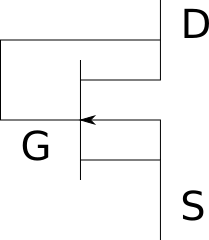
\includegraphics[width=0.25\textwidth]{./img/nmos-resistor}
\\\\
Motstanden blir da
$$R = \frac{V_{DS}}{I_D}$$
Motstanden er, som regel, i kilo-ohm og strømmen i milli-ampere.



\paragraph{NAND} \mbox \\
Man kan implementere unipolare logiske kretser med NMOS.
\\
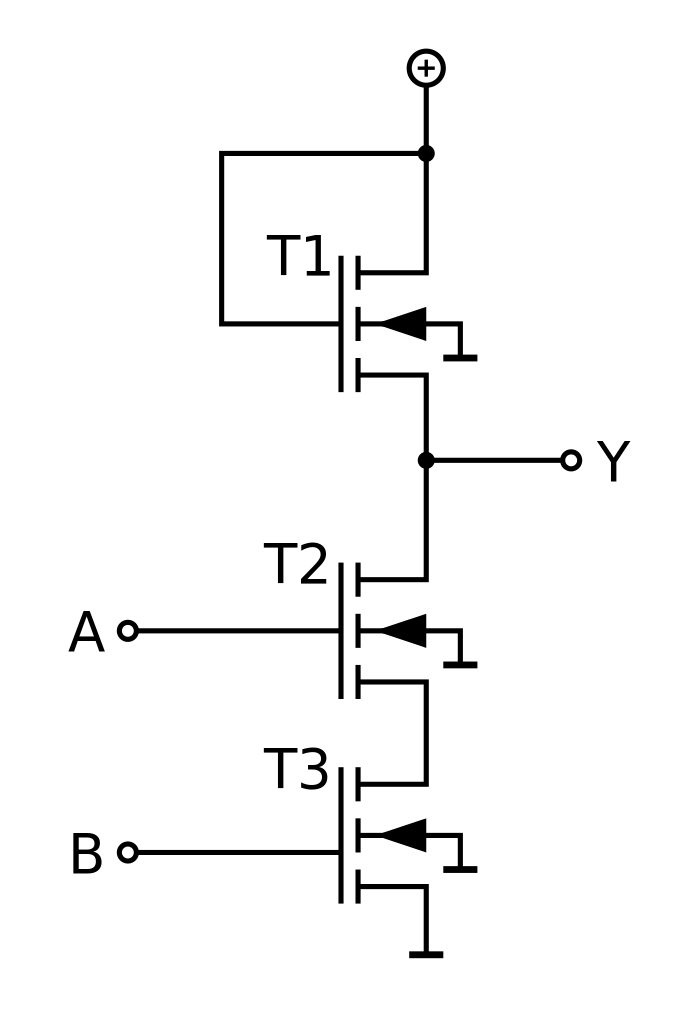
\includegraphics[width=0.5\textwidth]{./img/nmos-nand}
\\
Sannhetstabellen blir lik NAND i forige seksjon.
Når både A og B er på vil transistoren lede.
Når transistoren leder vil Y bringes ned til jord AKA null.



\paragraph{NOR} \mbox \\
NOR port implementert med NMOS.
\\
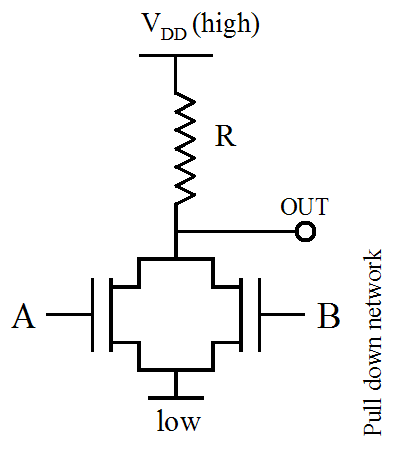
\includegraphics[width=0.5\textwidth]{./img/nmos-nor}
\\
På bildet kan man bytte ut R med en nmos-motstand (gate og drain koblet).

Hvis minst én av A eller B er på, vil transistoren lede.
Når en eller begge transistorene leder, bringes Y til jord.
